\subsection{Heuristic Methods}\label{heuristic}
Heuristic optimization methods often rely on different predefined rules or even trial and error when seeking the solution of an optimization problem. These methods usually do not guarantee optimal solutions, but they are often effective for finding near-optimal results in a reasonable amount of time. Heuristic methods include genetic algorithms, detailed in \cite{BBO-textbook}, along with various other heuristic approaches.

In this section, however, we will focus on a different widely used heuristic method, the Nelder-Mead method, also known as the simplex method\footnote{A simplex in $ \mathbb{R}^n $ is defined as a bounded convex polytope (a generalization of a polyhedron to any dimension) with a non-empty interior and exactly $ n+1 $ vertices \cite{BBO-textbook}.}\footnote{The term "simplex method" more commonly refers to the algorithm used to find the optimal solution in linear programming. This algorithm was developed by George Dantzig \cite{Dantzig1990}.}\cite{Nelder1965}.

The Nelder-Mead method finds a solution to an optimization problem by iteratively constructing simplexes. The process begins by initializing a starting simplex. The objective function is then evaluated at each vertex of this simplex. In each subsequent iteration, the simplex is transformed in order to move closer to the position of the sought stationary point of the objective function. The transformation of the simplex involves manipulating its points using predefined operations -- expansion, reflection, contraction (inner and outer), and shrinking, which are schematically illustrated in Figure~\ref{fig:NM operations}. 

\begin{figure}[H]
	%	\vspace{5mm}
	\centering
	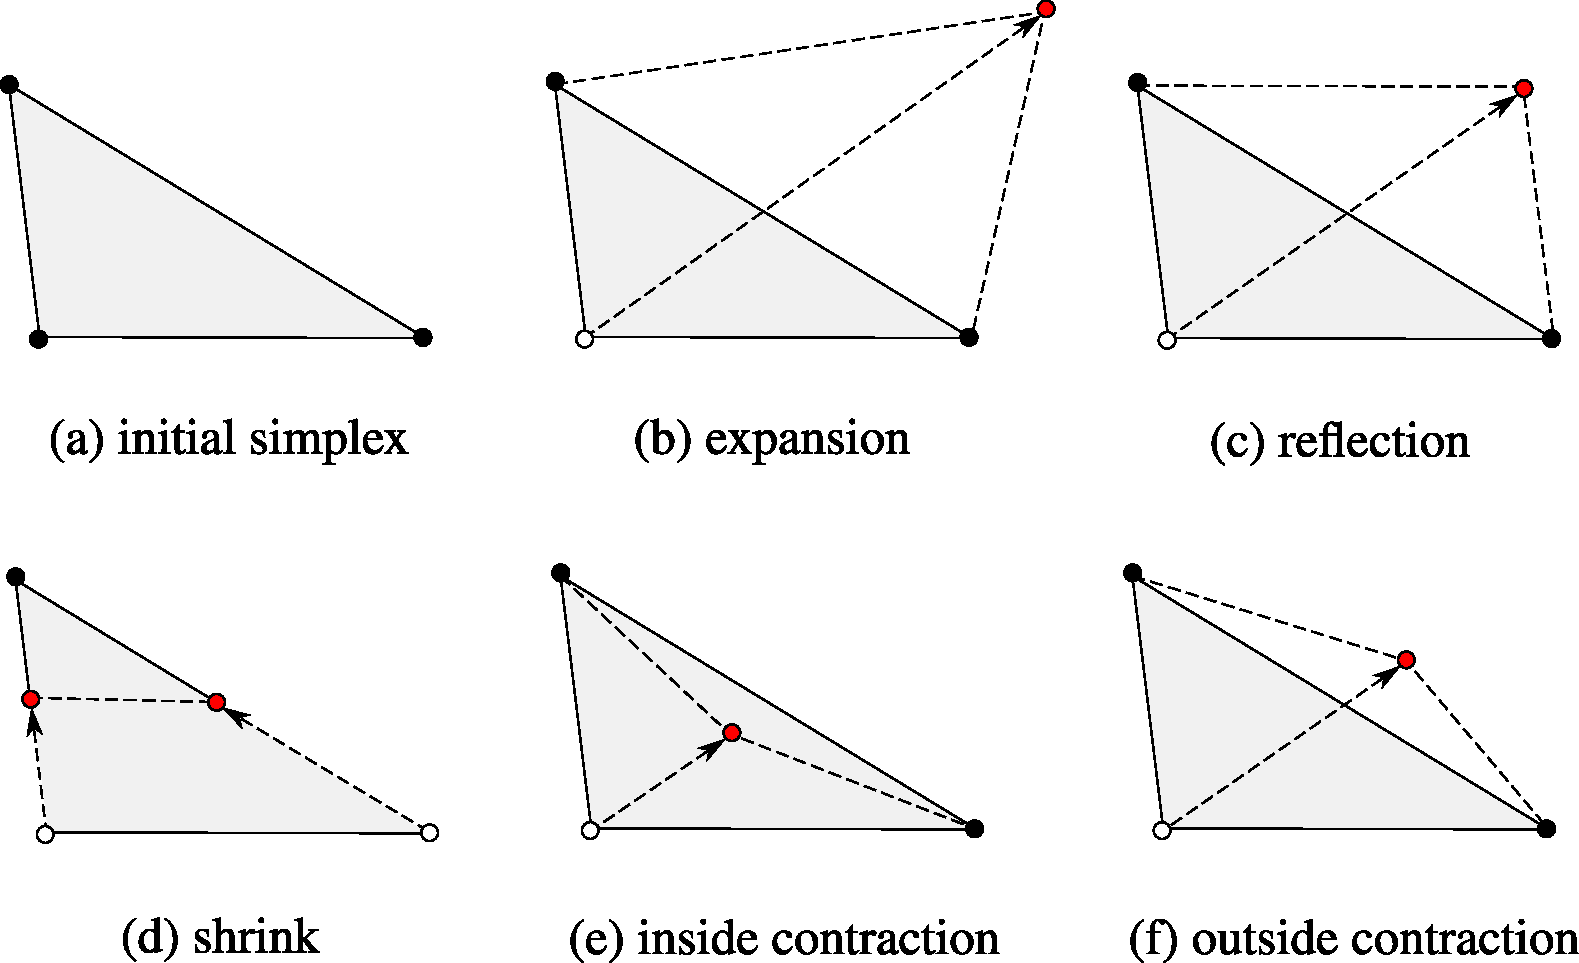
\includegraphics[width=0.96\textwidth]{figures/neldermead.pdf}
	\vspace{2mm}
	\caption{A schematic representation of the operations used to transform simplexes in the Nelder-Mead method. The vertices generated by applying each operation are shown in red. For clarity, the operations are depicted in $ \mathbb{R}^2 $.}
	%	\vspace{2mm}
	\label{fig:NM operations}
\end{figure}

The transformations performed during each iteration are determined by comparing the function values at the vertices of the simplex. The newly formed simplex shares either exactly one vertex or exactly $ n $ vertices with the simplex from the preceding iteration. The algorithm continues to iteratively transform the simplex until a stopping condition (specified by the user) is met \cite{BBO-textbook}. Details of the Nelder-Mead method, including the algorithm's description and the choice of stopping condition, are discussed in \cite{BBO-textbook, derivative-free-review, Nelder1965}. The full Nelder-Mead method algorithm is presented in Algorithm~\ref{neldermead}.

\begin{algorithm}
	\caption{Nelder-Mead algorithm}\label{neldermead}
	\begin{algorithmic}[1]
		\Require Initial simplex $S^0 = \{s^0, s^1, \dots, s^n\}$, function $f: \mathbb{R}^n \to \mathbb{R}$, parameters $\delta^{\text{e}}$, $\delta^{\text{oc}}$, $\delta^{\text{ic}}$, $\gamma$, iteration counter $k \gets 0$
		\Ensure Approximate optimal solution $\vec{x^{\star}}$ for function $f$
		
		\Procedure{Nelder-Mead}{$S^0$}
		\State Reorder $S^k$ so that $f(s^0) \leq f(s^1) \leq \dots \leq f(s^n)$
		\State Set $f^k_{\text{best}} = f(s^0)$
		
		\While{stopping condition not met}
		\Algphase{Reflection}
		\State Compute centroid $x^{\text{c}} = \frac{1}{n} \sum_{i=0}^{n-1} s^i$
		\State Set reflection point $x^{\text{r}} = x^{\text{c}} + (x^{\text{c}} - s^n)$ and compute $f^{\text{r}} = f(x^{\text{r}})$
		\If{$f^k_{\text{best}} \leq f^{\text{r}} < f(s^{n-1})$}
		\State Set $S^{k+1} = \{s^0, s^1, \dots, s^{n-1}, x^{\text{r}}\}$
		\State Increment $k \gets k+1$ and continue
		\EndIf
		
		\Algphase{Expansion}
		\If{$f^{\text{r}} < f^k_{\text{best}}$}
		\State Set expansion point $x^{\text{e}} = x^{\text{c}} + \delta^{\text{e}} (x^{\text{r}} - x^{\text{c}})$ and compute $f^{\text{e}} = f(x^{\text{e}})$
		\If{$f^e < f^r$}
		\State Set $S^{k+1} = \{s^0, s^1, \dots, s^{n-1}, x^\text{e}\}$
		\Else
		\State Set $S^{k+1} = \{s^0, s^1, \dots, s^{n-1}, x^\text{r}\}$
		\EndIf
		\State Increment $k \gets k+1$ and continue
		\EndIf
		
		\Algphase{Contraction}
		\If{$f^\text{r} \geq f(s^n)$}
		\State \textbf{Outside Contraction:} Compute $x^\text{oc} = x^\text{c} + \delta^{\text{oc}}(x^\text{c} - s^n)$ and $f^{\text{oc}} = f(x^{\text{oc}})$
		\If{$f^{\text{oc}} < f(s^n)$}
		\State Set $S^{k+1} = \{s^0, s^1, \dots, s^{n-1}, x^{\text{oc}}\}$
		\Else
		\State \textbf{Shrink:} Set $S^{k+1} = \{s^0, s^0 + \gamma(s^1 - s^0), \dots, s^0 + \gamma(s^n - s^0)\}$
		\EndIf
		\State Increment $k \gets k+1$ and continue
		\Else
		\State \textbf{Inside Contraction:} Compute $x^{\text{ic}} = x^\text{c} + \delta^{\text{ic}}(x^\text{c} - s^n)$ and $f^{\text{ic}} = f(x^{\text{ic}})$
		\If{$f^{\text{ic}} < f(s^n)$}
		\State Set $S^{k+1} = \{s^0, s^1, \dots, s^{n-1}, x^{\text{ic}}\}$
		\Else
		\State Set $S^{k+1} = \{s^0, s^0 + \gamma(s^1 - s^0), \dots, s^0 + \gamma(s^n - s^0)\}$
		\EndIf
		\State Increment $k \gets k+1$ and continue
		\EndIf
		\EndWhile
		\EndProcedure
	\end{algorithmic}
\end{algorithm}
%
The heuristic nature of the Nelder-Mead method stems from the fact that its principle is based on a somewhat random search of the space using predefined rules. Several iterations of space exploration using simplexes, for a specific choice of initial simplex and a specific function, are shown in Figure \ref{fig:NM}. While the convergence of this method has been proven, it is not guaranteed that the method will always converge to a stationary point \cite{BBO-textbook}. It should be noted that the Nelder-Mead method was primarily developed for unconstrained optimization problems, but it can be adapted for constrained optimization problems  \cite{BBO-textbook}.


\begin{figure}[H]
	\vspace{-5mm}
	\begin{subfigure}[b]{0.325\textwidth}
		\centering
		%		trim={<left> <lower> <right> <upper>}
		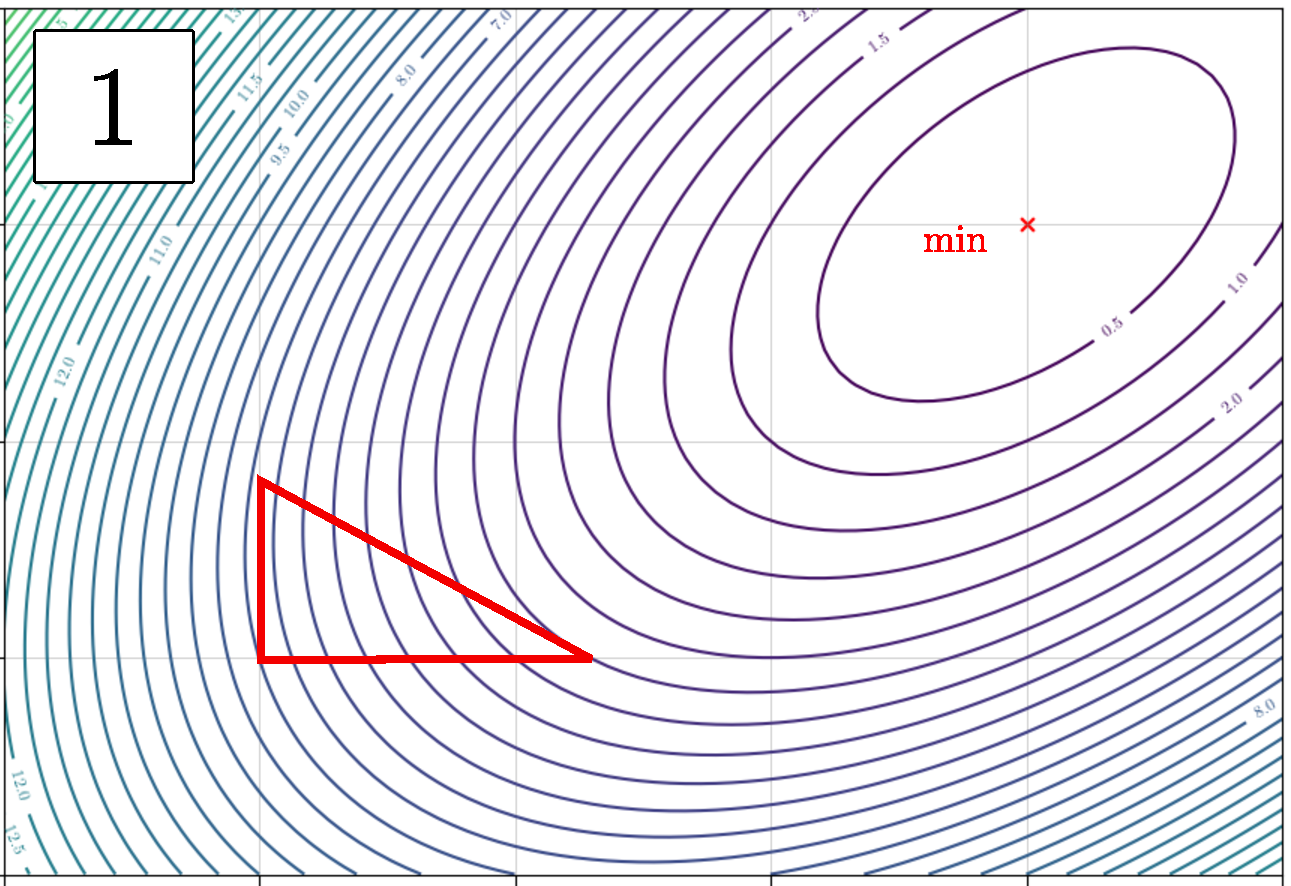
\includegraphics[width=0.96\textwidth, trim={0 0 0 0}, clip]{figures/nelder1.pdf}
	\end{subfigure}
	\begin{subfigure}[b]{0.325\textwidth}
		\centering
		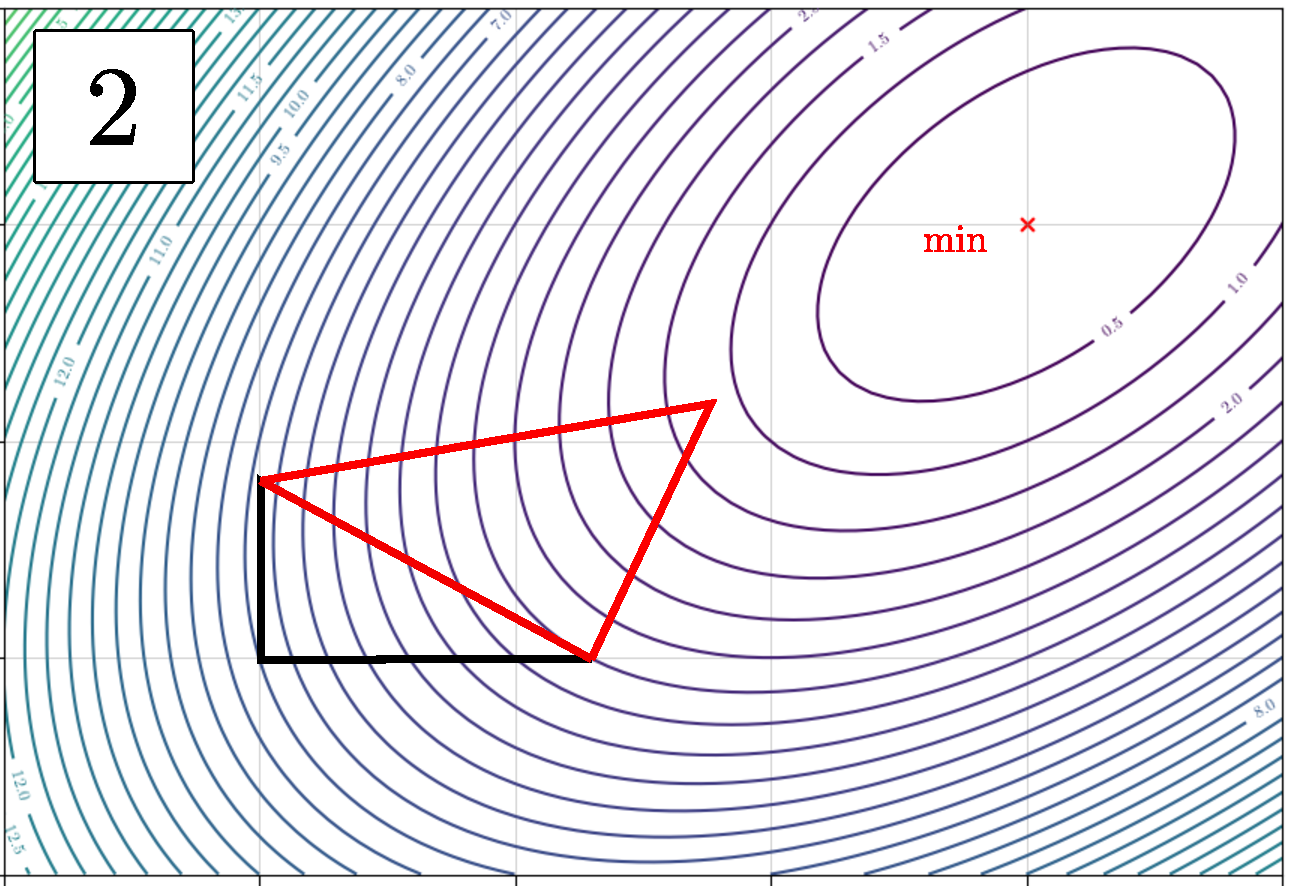
\includegraphics[width=0.96\textwidth, trim={0 0 0 0}]{figures/nelder2.pdf}
	\end{subfigure}
	\vspace{1mm}
	\begin{subfigure}[b]{0.325\textwidth}
		\centering
		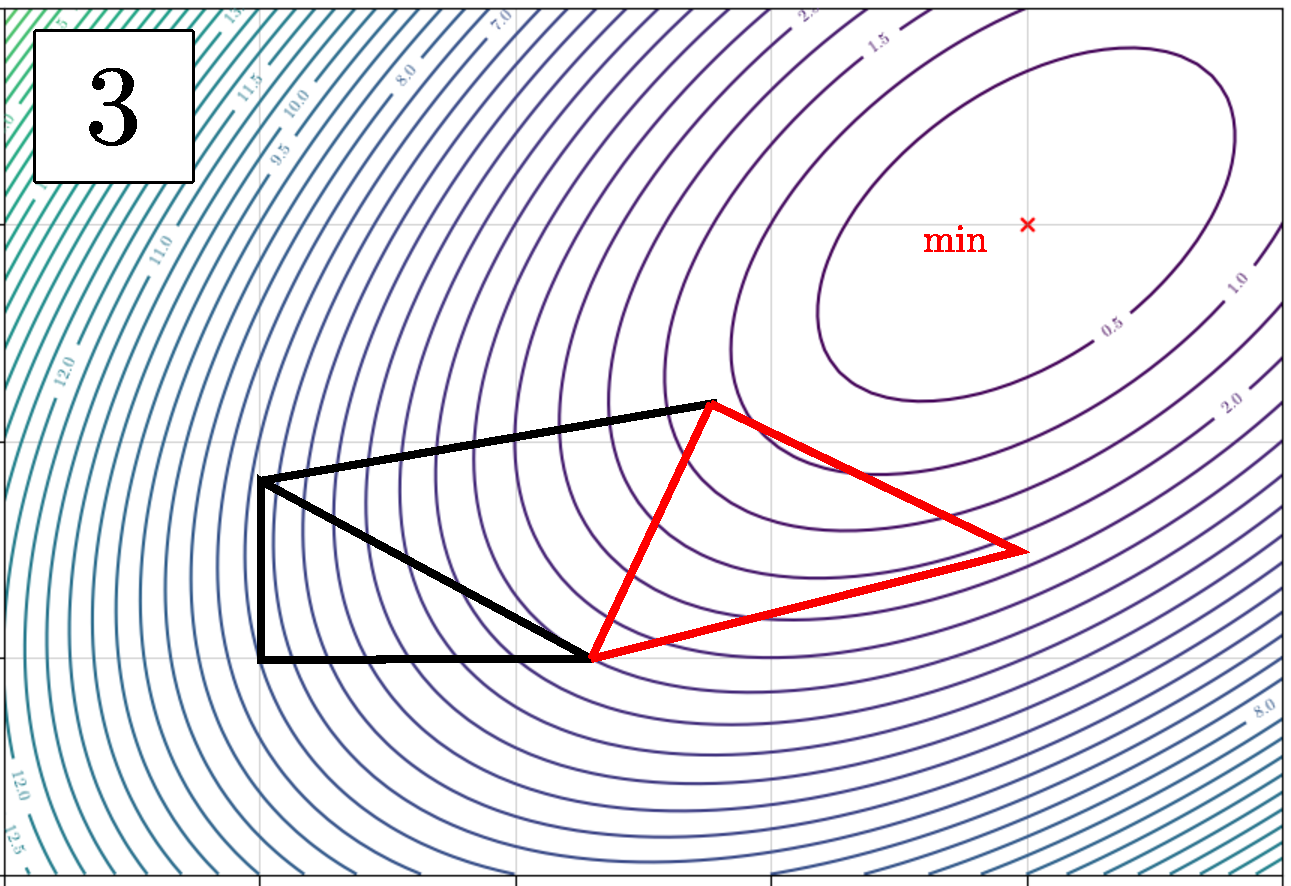
\includegraphics[width=0.96\textwidth, trim={0 0 0 0}]{figures/nelder3.pdf}
	\end{subfigure}
	\vspace{1mm}
	\begin{subfigure}[b]{0.325\textwidth}
		\centering
		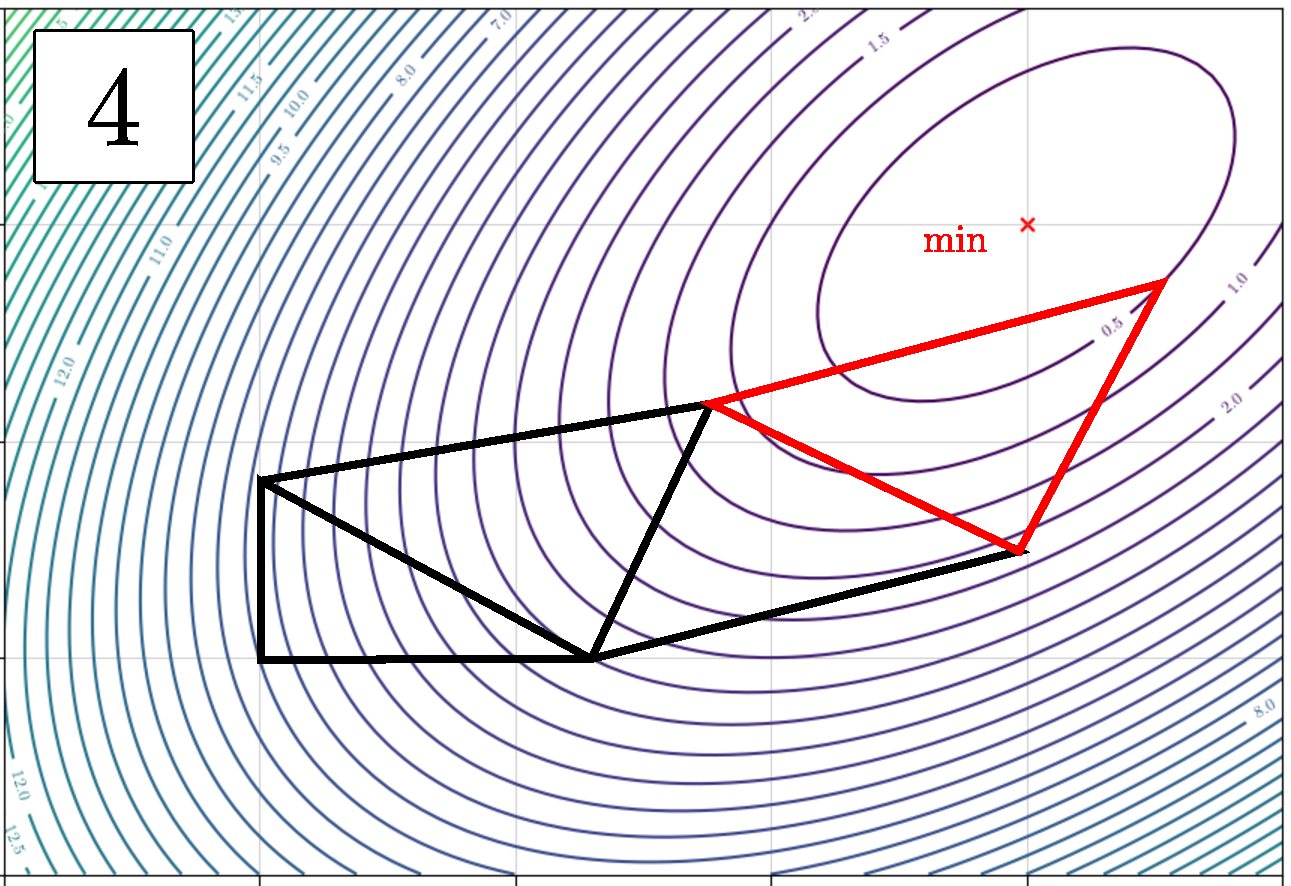
\includegraphics[width=0.96\textwidth, trim={0 0 0 0}]{figures/nelder4.pdf}
	\end{subfigure}
	\begin{subfigure}[b]{0.325\textwidth}
		\centering
		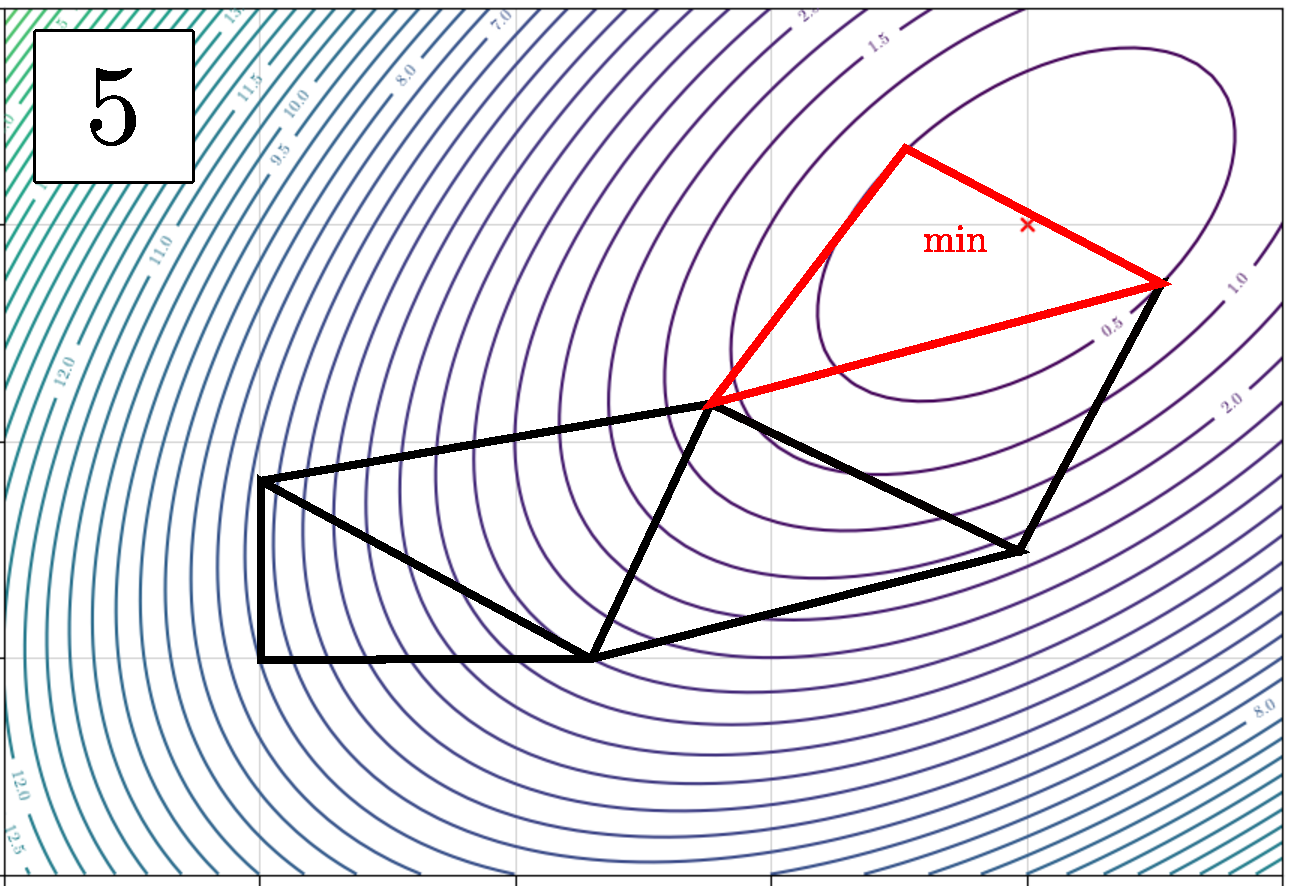
\includegraphics[width=0.96\textwidth, trim={0 0 0 0}]{figures/nelder5.pdf}
	\end{subfigure}
	\begin{subfigure}[b]{0.325\textwidth}
		\centering
		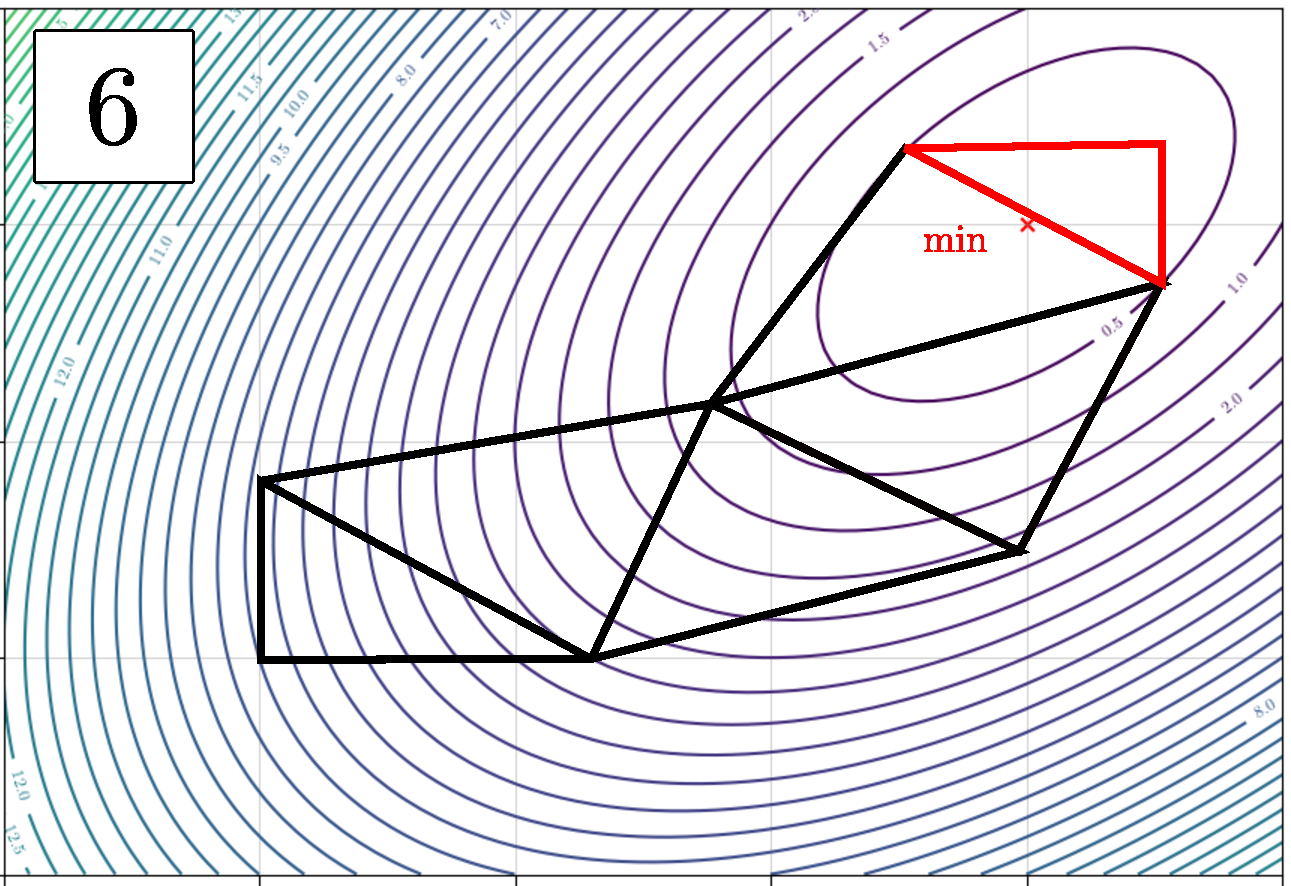
\includegraphics[width=0.96\textwidth, trim={0 0 0 0}]{figures/nelder6.pdf}
	\end{subfigure}
	\centering
	\begin{subfigure}[b]{0.325\textwidth}
		\centering
		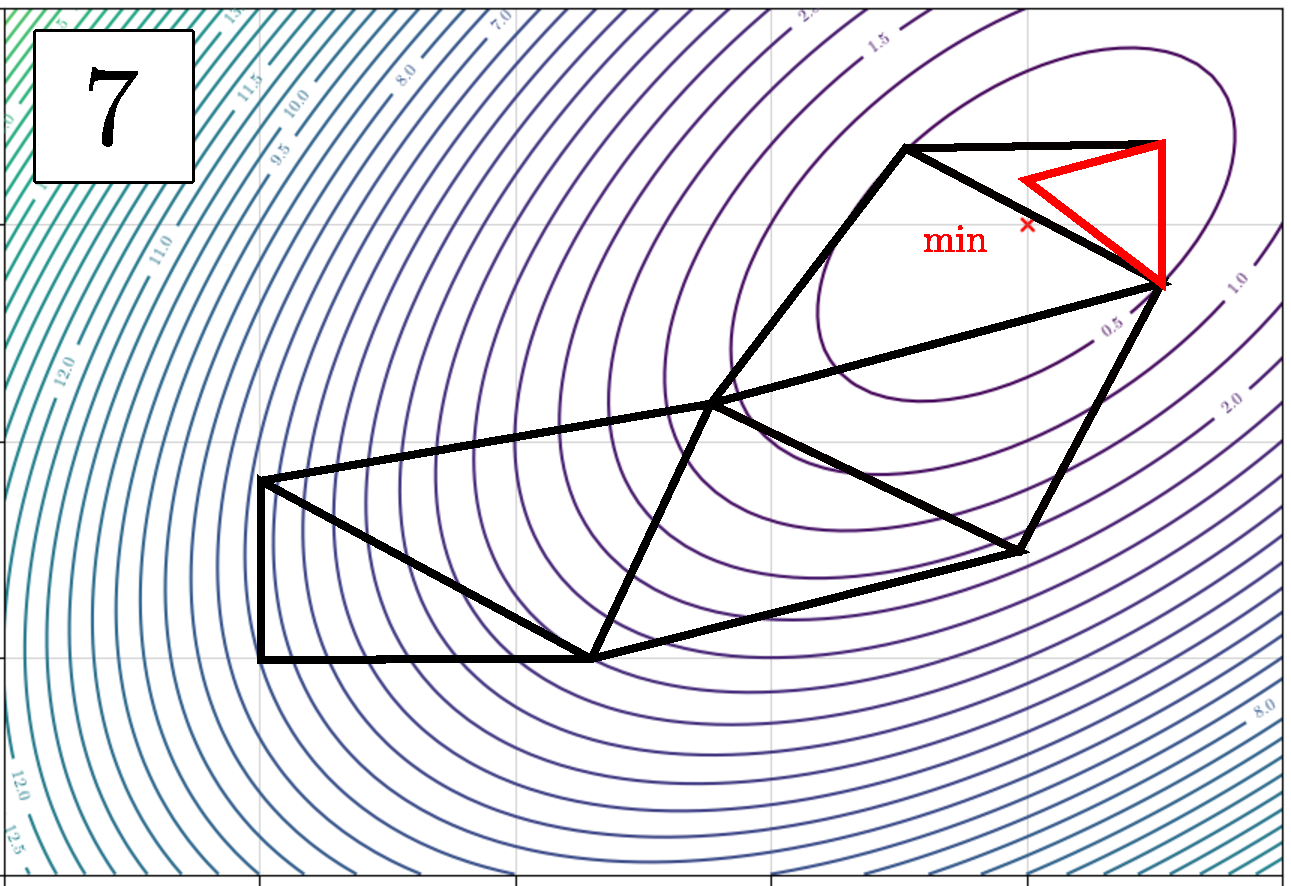
\includegraphics[width=0.96\textwidth, trim={0 0 0 0}]{figures/nelder7.pdf}
	\end{subfigure}
	\begin{subfigure}[b]{0.325\textwidth}
		\centering
		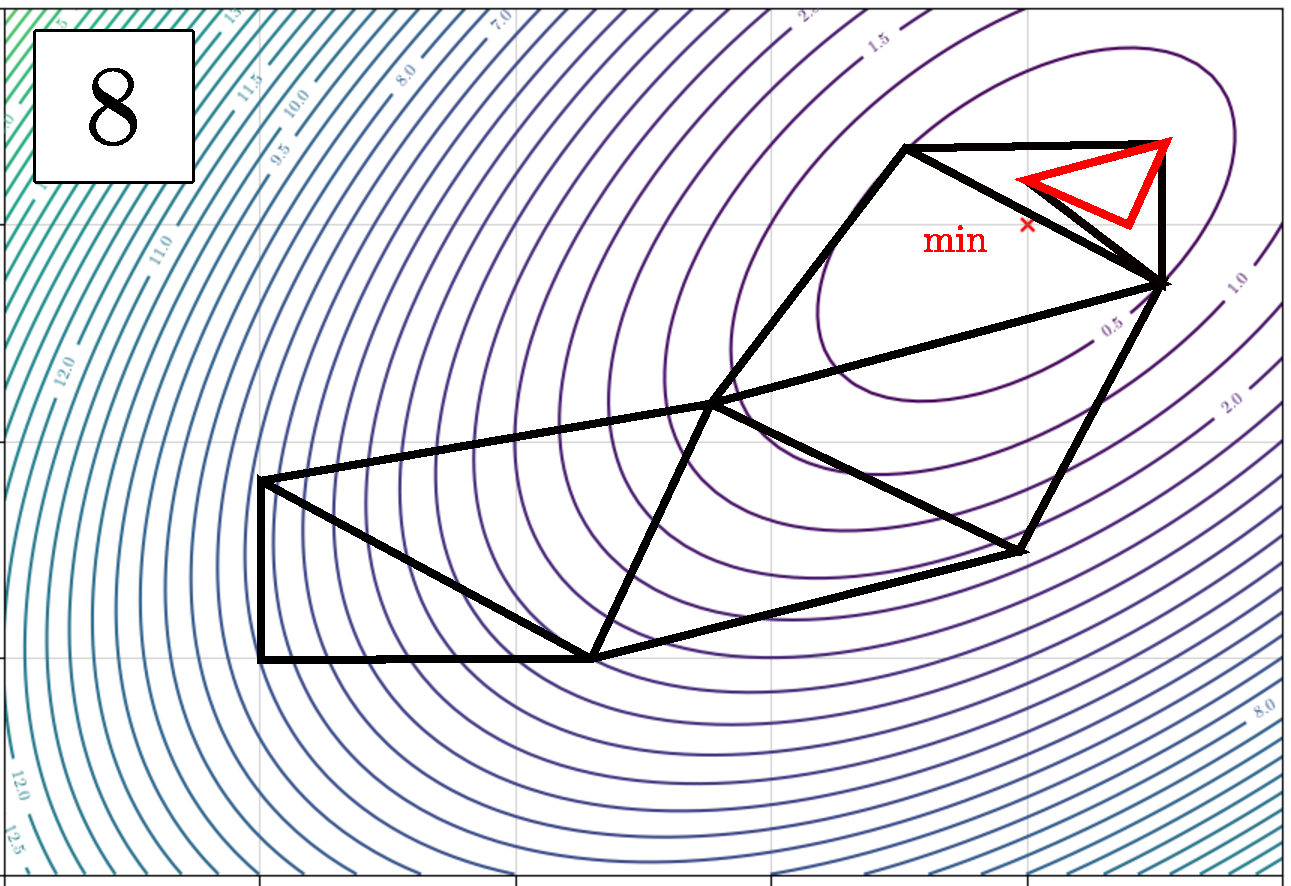
\includegraphics[width=0.96\textwidth, trim={0 0 0 0}]{figures/nelder8.pdf}
	\end{subfigure}
	\begin{subfigure}[b]{0.325\textwidth}
		\centering
		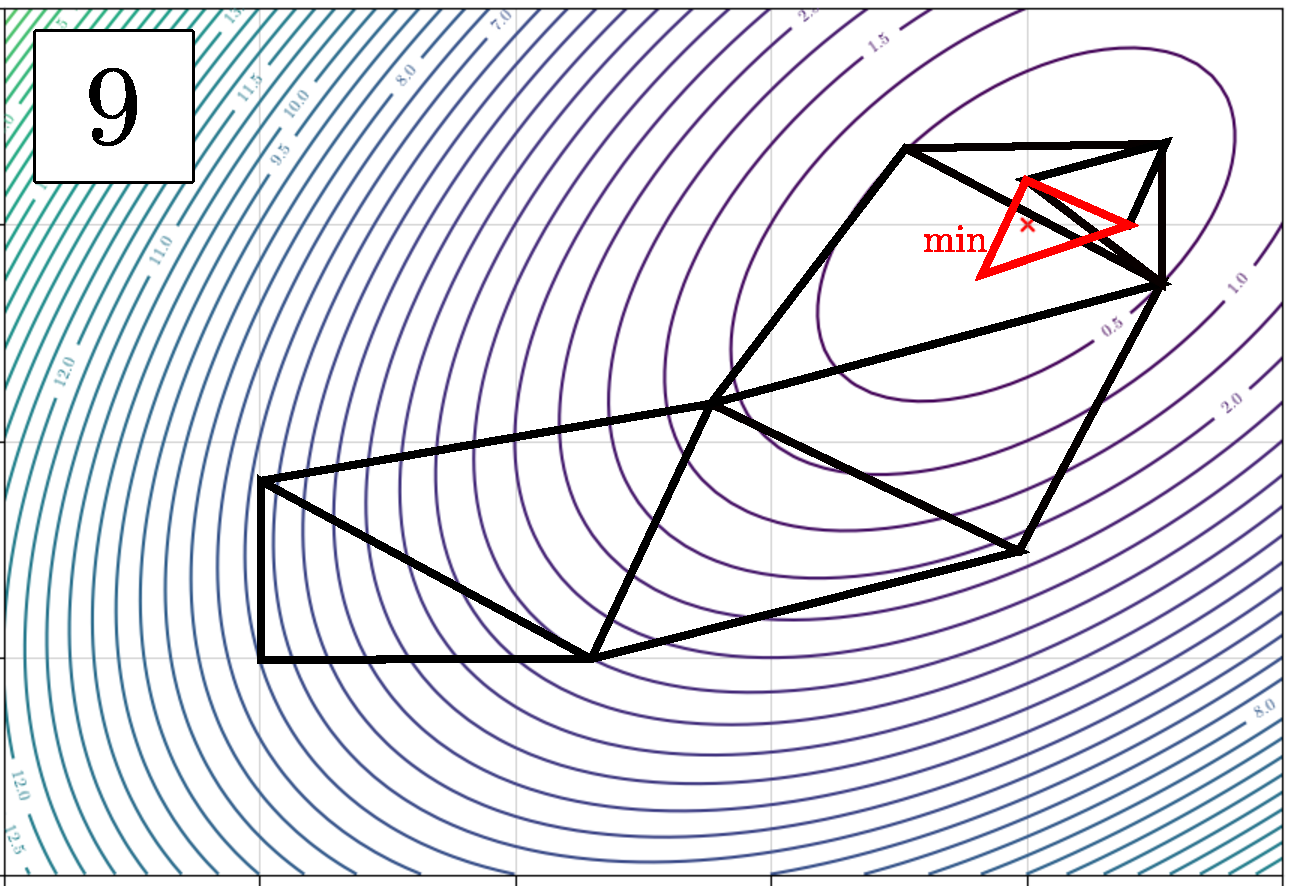
\includegraphics[width=0.96\textwidth, trim={0 0 0 0}]{figures/nelder9.pdf}
	\end{subfigure}
	\begin{center}
		\begin{subfigure}[b]{0.77\textwidth}
			\centering
			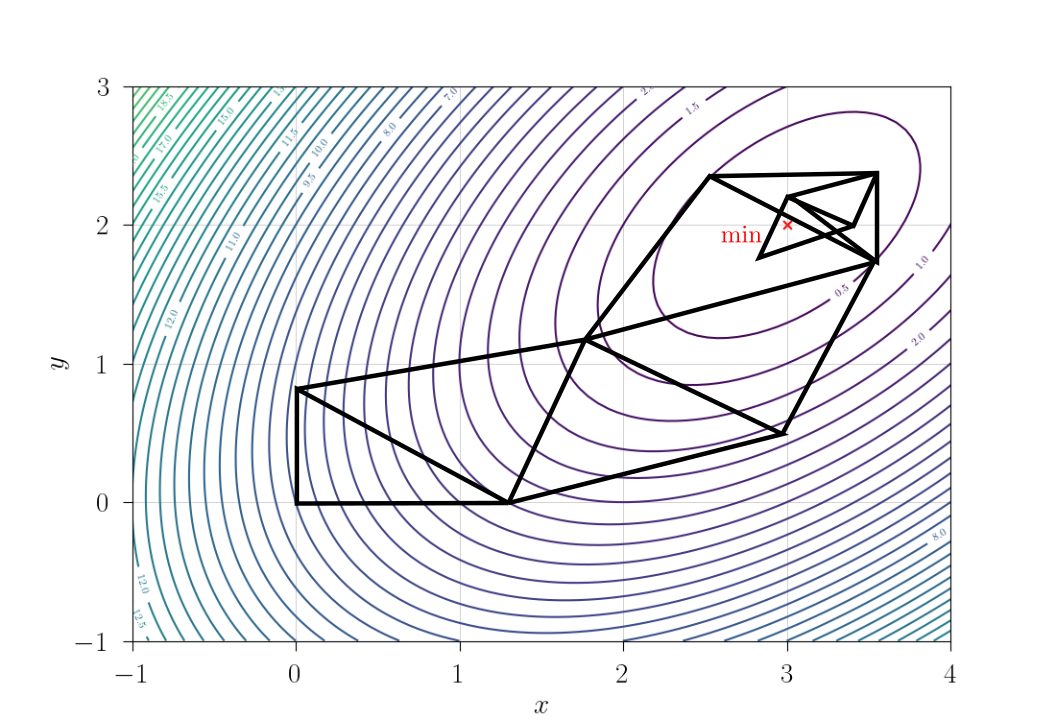
\includegraphics[width=0.985\textwidth, trim={0 6mm 0 7mm}]{figures/nelder.png}
		\end{subfigure}
	\end{center}
	
	\caption{Several iterations of the Nelder-Mead method for a specific choice of the initial simplex when minimizing the function $ x^2 - 4x + y^2 - y - xy + 7 $, with the minimum at the point (3,2) marked by a red cross.}
	\label{fig:NM}
\end{figure}

